\documentclass[aspectratio=169]{beamer}
\usetheme{Boadilla}
\usepackage[T1]{fontenc}
\usepackage{lmodern}
\usepackage{booktabs}
\usepackage{pgfplots}
\pgfplotsset{compat=1.18}
\setbeamertemplate{navigation symbols}{}

% Edit the title block. The short forms in [brackets] appear in the footer.
\title[Adaptive Caching]{Adaptive Caching for Edge Inference}
\subtitle{Cutting latency without extra hardware}
\author[A. Rivera]{Alex Rivera, Sam Okafor}
\institute[Northfield Univ.]{Systems Lab, Northfield University}
\date[SysConf 2026]{SysConf 2026, Session 4B}

\begin{document}

\begin{frame}
  \titlepage
\end{frame}

\begin{frame}{Outline}
  \tableofcontents
\end{frame}

\section{Motivation}
\begin{frame}{Why this matters}
  \begin{columns}[T]
    \begin{column}{0.55\textwidth}
      \begin{itemize}
        \item Edge devices repeat many near identical requests.
        \item Recomputing each one wastes energy and time.
        \item Existing caches ignore how inputs drift over a day.
      \end{itemize}
      \vspace{1em}
      \begin{alertblock}{Research question}
        Can a cache that adapts to drift keep accuracy while halving latency?
      \end{alertblock}
    \end{column}
    \begin{column}{0.4\textwidth}
      \centering
      % Replace this box with your own TikZ figure or diagram.
      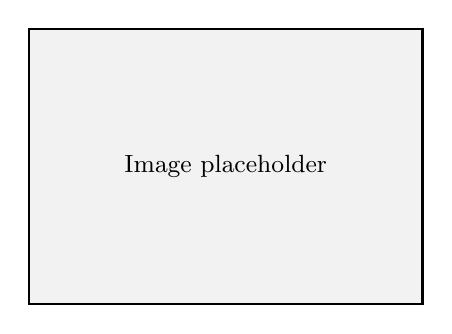
\begin{tikzpicture}
        \draw[thick, fill=gray!10] (0,0) rectangle (5,3.5);
        \node at (2.5,1.75) {\small Image placeholder};
      \end{tikzpicture}
    \end{column}
  \end{columns}
\end{frame}

\section{Method}
\begin{frame}{Approach in three steps}
  \begin{enumerate}
    \item \textbf{Embed} each request into a compact key.
    \item \textbf{Match} the key against recent entries with a similarity threshold.
    \item \textbf{Adapt} the threshold online from observed error.
  \end{enumerate}
  \vspace{1em}
  \centering
  \begin{tikzpicture}[box/.style={draw, rounded corners, fill=structure.fg!15, minimum width=2.6cm, minimum height=0.9cm}]
    \node[box] (a) at (0,0) {Request};
    \node[box] (b) at (3.5,0) {Key lookup};
    \node[box] (c) at (7,0.8) {Cache hit};
    \node[box] (d) at (7,-0.8) {Run model};
    \draw[->, thick] (a) -- (b);
    \draw[->, thick] (b) -- (c);
    \draw[->, thick] (b) -- (d);
  \end{tikzpicture}
\end{frame}

\section{Results}
\begin{frame}{Latency and accuracy}
  \begin{columns}[c]
    \begin{column}{0.48\textwidth}
      % Edit the numbers in the table rows below.
      \begin{tabular}{lrr}
        \toprule
        Method & Latency (ms) & Accuracy \\
        \midrule
        No cache & 84 & 91.2\% \\
        Fixed cache & 51 & 88.7\% \\
        \textbf{Ours} & \textbf{39} & \textbf{90.9\%} \\
        \bottomrule
      \end{tabular}
    \end{column}
    \begin{column}{0.48\textwidth}
      \centering
      % Change the coordinates to plot your own values.
      \begin{tikzpicture}
        \begin{axis}[
            ybar, width=6.5cm, height=4.5cm,
            symbolic y coords={No cache,Fixed cache,Ours},
            ytick=data, xmin=0, xlabel={Latency (ms)},
            point meta=x, nodes near coords, bar width=10pt,
            enlarge y limits=0.3]
          \addplot[fill=structure.fg!70] coordinates {(84,No cache) (51,Fixed cache) (39,Ours)};
        \end{axis}
      \end{tikzpicture}
    \end{column}
  \end{columns}
\end{frame}

\begin{frame}{What we learned}
  \begin{block}{Key finding}
    Adapting the threshold recovers almost all accuracy lost by a fixed cache.
  \end{block}
  \begin{exampleblock}{Where it helps most}
    Workloads with slow drift, such as camera feeds and voice commands.
  \end{exampleblock}
\end{frame}

\section{Conclusion}
\begin{frame}{Conclusion}
  \begin{itemize}
    \item 54\% lower latency than no cache, with accuracy within 0.3 points.
    \item Works on unmodified hardware.
    \item Code and data: \texttt{example.org/adaptive-cache}
  \end{itemize}
  \vspace{2em}
  \centering
  {\Large Thank you. Questions?}
\end{frame}

\appendix
\section*{Backup}
\begin{frame}{Backup: threshold sensitivity}
  \begin{tabular}{lccc}
    \toprule
    Threshold & 0.80 & 0.90 & 0.95 \\
    \midrule
    Hit rate & 71\% & 58\% & 40\% \\
    Accuracy & 87.1\% & 90.2\% & 91.0\% \\
    \bottomrule
  \end{tabular}
\end{frame}

\begin{frame}{Backup: experimental setup}
  \begin{itemize}
    \item Device: 4 core ARM board, 4 GB memory.
    \item Model: 12 layer vision transformer, 8 bit weights.
    \item Traces: 14 days of recorded requests from three sites.
  \end{itemize}
\end{frame}

\end{document}
